% ============================================================
%  THEORETICAL BACKGROUND — IEEE VSSS DOMAIN
%  Complete text for the three sections.
%  (The first two sections are lightly revised from your draft;
%   the third is written from scratch.)
% ============================================================

This chapter covers the IEEE VSSS domain, the differential-drive robot model, and the existing simulators used in the community, identifying the architectural constraints that motivate the GPU-accelerated approach taken in this work.

% ------------------------------------------------------------------
\section{The IEEE VSSS Domain}
% ------------------------------------------------------------------

IEEE Very Small Size Soccer (\gls{vsss}) is a Robot Soccer category in which two teams
of small differential-drive robots compete on a flat field.  The robots are
remotely controlled by a computer set by each team that receives the state of the
game from a camera set over the field and sends wheel-speed commands by radio~\parencite{robocore_vsss_rules}.  Human
intervention is not allowed during regular play, so the control system must
close the loop from perception to decision-making and actuation.

Compared with larger Robot Soccer leagues, \gls{vsss} has relatively simpler
physics: rigid (no geometry-altering controllable joints) robots, a ball, wall collisions, friction, and no kicking
mechanism.  This simplicity makes the domain specially attractive for reinforcement
learning because it can be simulated at high computational efficiency.
At the same time, the task is not trivial: a team must conduct the ball by contact, coordinate the motion of multiple robots, avoid blocking itself, defend its goal, and exploit opportunities created by the opponent.

The match for a 3v3 category variant takes place on a rectangular field of dimensions
$1.50\,\text{m} \times 1.30\,\text{m}$ (excluding the goal areas), with one
goal centered on each of the shorter sides.  Figure~\ref{fig:field} shows the
regulation layout for the 3v3 field in centimetres (goals, penalty areas, centre circle, and chamfered corners).  An overhead camera feeds a vision system that estimates the position of the ball and the pose (position and orientation) of every robot; those estimates are then consumed by the decision-making stack (strategy, path planning, and low-level control).
In real hardware, the whole pipeline (vision and decision-making) runs inside a computer set by each team that
issues wheel-speed commands over radio, so all computation is centralized.

\begin{figure}[ht]
    \centering
    \resizebox{0.88\linewidth}{!}{%
        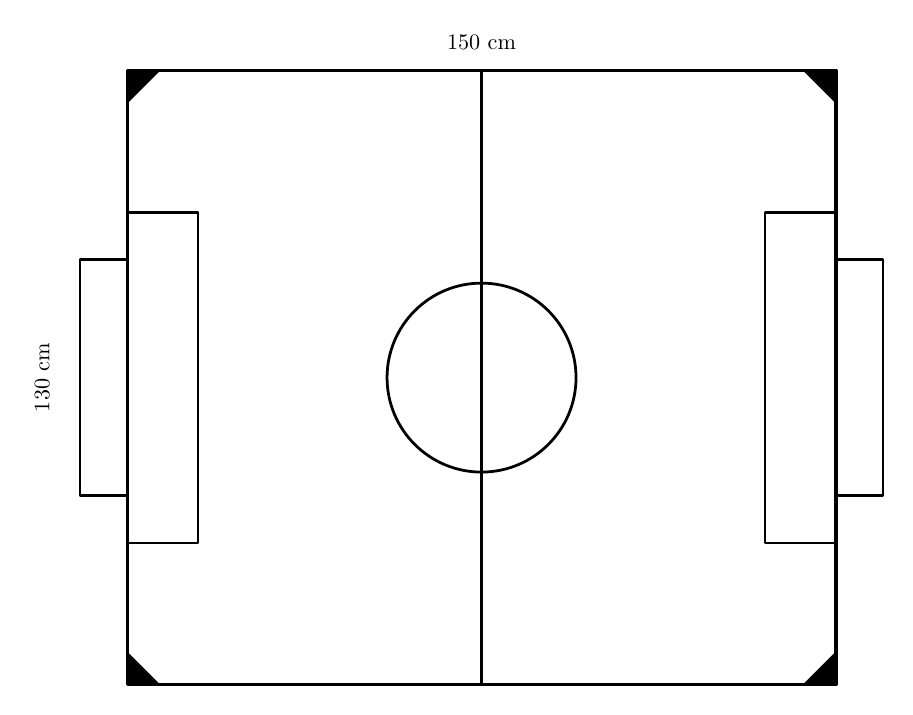
\begin{tikzpicture}[scale=0.06, line cap=round, line join=round]

  % Dimensions: field 150cm x 130cm
  \def\W{150}
  \def\H{130}
  
  % Outer field
  \draw[line width=1.2pt] (0,0) rectangle (\W,\H);
  
  % Chamfered black corners, 7cm
  \foreach \x/\y/\xa/\ya/\xb/\yb in {
  0/0/7/0/0/7,
  150/0/143/0/150/7,
  0/130/7/130/0/123,
  150/130/143/130/150/123}
  {
    \fill (\x,\y) -- (\xa,\ya) -- (\xb,\yb) -- cycle;
  }
  
  % Center line
  \draw[line width=1pt] (75,0) -- (75,\H);
  
  % Center circle, diameter 40cm
  \draw[line width=1pt] (75,65) circle (20);
  
  % Goals
  \draw[line width=1pt] (-10,40) rectangle (0,90);
  \draw[line width=1pt] (\W,40) rectangle (\W+10,90);
  
  % Goal areas / boxes
  \draw[line width=1pt] (0,30) rectangle (15,100);
  \draw[line width=1pt] (\W-15,30) rectangle (\W,100);
  
% --- Penalty arcs via circumcenter / 3 points ---

% Left arc: start (20,55), through (15,65), end (20,75)
\tkzDefPoint(15,55){LA}
\tkzDefPoint(20,65){LB}
\tkzDefPoint(15,75){LC}
\tkzCircumCenter(LA,LB,LC)\tkzGetPoint{LO}
\tkzDrawArc[line width=1pt](LO,LA)(LC)

% Right arc: start (130,75), through (135,65), end (130,55)
\tkzDefPoint(135,75){RA}
\tkzDefPoint(130,65){RB}
\tkzDefPoint(135,55){RC}
\tkzCircumCenter(RA,RB,RC)\tkzGetPoint{RO}
\tkzDrawArc[line width=1pt](RO,RA)(RC)
  
  % Small marks / dots
  % \foreach \x/\y in {
  % 17.5/25, 57.5/25,
  % 17.5/105, 57.5/105,
  % 92.5/25, 132.5/25,
  % 92.5/105, 132.5/105}
  % {
  %   \draw[line width=0.8pt] (\x,\y) circle (1.2);
  % }
  
  % Cross markers
  % \foreach \x/\y/\txt in {
  % 37.5/25/{\textbf{\color{red}(FB)}},
  % 37.5/65/{\textbf{\color{red}(PK, FK)}},
  % 37.5/105/{\textbf{\color{red}(FB)}},
  % 112.5/25/{\textbf{\color{red}(FB)}},
  % 112.5/65/{\textbf{\color{red}(PK, FK)}},
  % 112.5/105/{\textbf{\color{red}(FB)}}}
  % {
  %   \draw[line width=1pt] (\x-2,\y) -- (\x+2,\y);
  %   \draw[line width=1pt] (\x,\y-2) -- (\x,\y+2);
  %   \node[scale=0.75] at (\x,\y+7) {\txt};
  % }
  
  % Optional coordinate labels
  \node[scale=0.8] at (75,136) {150 cm};
  \node[scale=0.8, rotate=90] at (-18,65) {130 cm};
  
  \end{tikzpicture}
%
    }
    \caption{IEEE VSSS field (top view, dimensions in cm).  Goals are
    $40$\,cm wide; penalty areas and centre markings follow the competition
    ruleset.}
    \label{fig:field}
\end{figure}

The 3v3 setting considered in this thesis increases the multi-agent nature
of the problem.  A single policy action can be evaluated only in the context
of the other allied robots and the opponent team.  This creates both
cooperative credit-assignment challenges and adversarial non-stationarity,
which the training methodology must address.

% ------------------------------------------------------------------
\section{Differential-Drive Robot Model}
% ------------------------------------------------------------------

Each \gls{vsss} robot can be modeled as a differential-drive body with two
independently actuated wheels.  A common kinematic mapping from body velocity
to wheel angular velocities~\cite{franzoni2017} is:

\begin{equation}
    \gls{wheel_speed_left} = \frac{2\gls{linear_velocity} - \gls{wheel_base}\,\gls{angular_velocity}}{\gls{wheel_diameter}},
    \qquad
    \gls{wheel_speed_right} = \frac{2\gls{linear_velocity} + \gls{wheel_base}\,\gls{angular_velocity}}{\gls{wheel_diameter}},
    \label{eq:diff_drive}
\end{equation}

where \gls{linear_velocity} is the desired linear velocity of the robot
center, \gls{angular_velocity} the desired angular velocity,
\gls{wheel_base} the distance between the wheel contact points,
\gls{wheel_diameter} the wheel diameter, and \gls{wheel_speed_left},
\gls{wheel_speed_right} the resulting left and right wheel angular
velocities.
This mapping is important because it defines the interface between the policy
and the simulator.  The policy may output wheel speeds directly, or it may
output higher-level $(v,\omega)$ commands that are converted into wheel
speeds before stepping the physics.  Direct wheel-speed actions are closer
to the hardware interface, while body-velocity actions can simplify learning
by exposing a more structured control space.

In the VSSS literature, both conventions have been used.
\cite{tg_thiago} and subsequent ITAndroids works adopt body
velocities as the policy output, converting them to wheel commands via
Equation~\eqref{eq:diff_drive} before dispatching to the simulator.
\cite{tg_thay} instead parameterize actions directly as a tuple of
left and right wheel speeds, arguing that the end-to-end formulation reduces
the gap between simulated commands and actual hardware actuation.  In either
case the robot is treated as a rigid cube that moves according to
Equation~\eqref{eq:diff_drive}, with friction and wall collisions handled by
the physics engine.

% ------------------------------------------------------------------
\section{Existing Simulators and Their Limitations for RL}
% ------------------------------------------------------------------

Because reinforcement learning algorithms require orders of magnitude more
interaction steps than classical approaches to converge, it is not practical
to train directly on physical hardware — doing so would quickly degrade the
robots' mechanical components and impose severe time constraints on
experimentation.  Simulation is therefore a necessary prerequisite, and the
choice of simulator has a direct bearing on how ambitious the training
methodology can be.

\subsection{The Conventional Architecture: ODE-Based Simulators}

The most established simulators in the VSSS community share a common
architectural pattern: a physics engine based on the \emph{Open Dynamics
Engine} (\gls{ode}). Written in C++, that runs as a standalone process and exposes
its state to external agents through socket messages.  ODE is an open-source
library for simulating rigid-body dynamics that requires only the geometry and
inertial parameters of each body as input, rather than manually derived
equations of motion \cite{smith2001}.  This makes it relatively
straightforward to replicate the VSSS scenario — a handful of cubic robots, a
spherical ball, and a bounded rectangular field.

Two simulators of this kind were mainly used in the VSSS analyzed works: the first,
developed by ITAndroids and used in prior works from the
group~\parencite{tg_thiago,tg_thay,master_thay}, combines ODE for physics
with the Object-Oriented Graphics Rendering Engine (OGRE) for visualization.
It operates at a fixed iteration rate of 60\,Hz and communicates with the
agent binaries through synchronous TCP socket packages built on the ZeroMQ
library.  To mimic real-world conditions, the simulator can inject additive
Gaussian noise into the position and orientation estimates it reports, and
can simulate communication delay by queuing observation packets and releasing
them with a configurable lag.  Figure~\ref{fig:itandroids_simulator} shows the
simulator rendering a penalty situation.

\begin{figure}[ht]
    \centering
    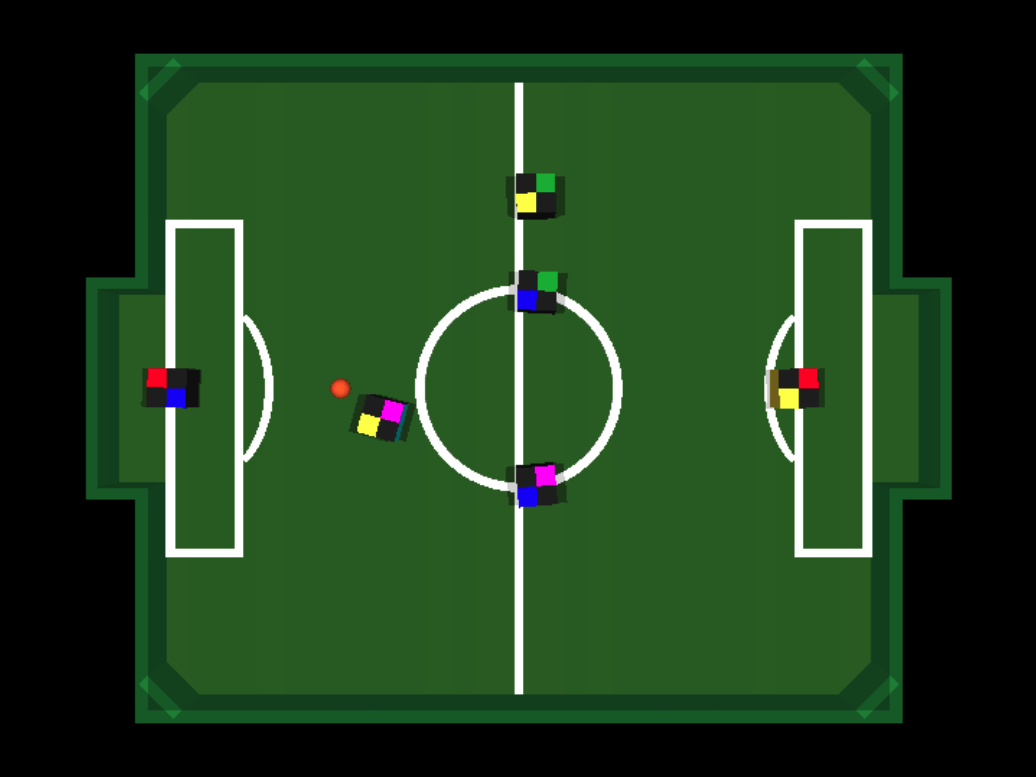
\includegraphics[width=0.82\linewidth]{Cap2/server.png}
    \caption{Screenshot of the ITAndroids ODE-based simulator in a penalty
    situation, with attacking and defending robots positioned around the ball.
    Image credit:~\parencite{master_thay}.}
    \label{fig:itandroids_simulator}
\end{figure}

The second, FIRASim~\cite{firasim2019}, was adapted from the RoboCup Small
Size League simulator grSim and is the reference environment used by many of the Brazilian VSSS simulated competitions.  It also uses ODE for
physics but is a different implementation, with known behavioral differences:
it does not enforce velocity limits on robots and omits friction in certain
contact configurations.  FIRASim uses asynchronous
UDP communication rather than TCP, and does not include built-in noise or delay injection.  Figure~\ref{fig:firasim} shows a FIRASim match state.

\begin{figure}[ht]
    \centering
    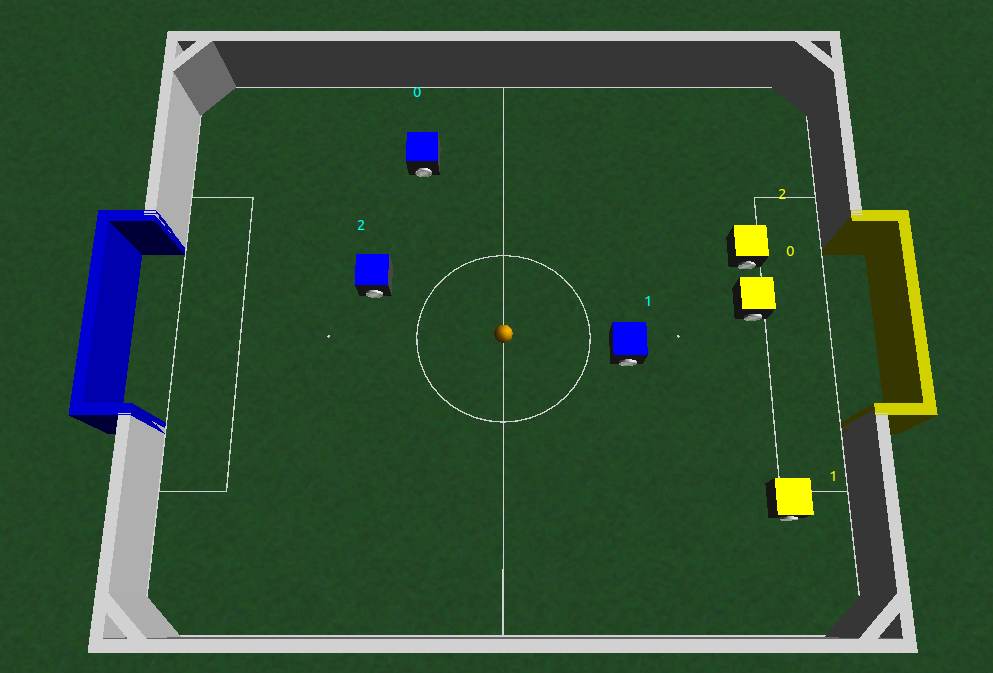
\includegraphics[width=0.82\linewidth]{Cap2/firasim.png}
    \caption{Screenshot of the FIRASim simulator, the ODE-based environment commonly used in Brazilian VSSS simulated competitions. Credit:~\parencite{firasim2019}.}
    \label{fig:firasim}
\end{figure}

Both simulators expose an interface in which the agent processes are entirely
separate from the physics process.  At each timestep, the simulator broadcasts
the current game state (robot poses, velocities, and ball state) to both teams,
waits for them to respond with desired wheel speeds, updates the physics, and
then repeats.  This synchronous, round-trip structure means that the simulator and the agent
processes are tightly coupled in time even though they run independently.
Gym-compatible wrappers have been built on
top of both engines to standardize the observation and action spaces and to
allow interchangeable use with general RL toolkits, following \parencite{bassani2020}.

\subsection{The Throughput Bottleneck}

The multi-process, socket-based architecture described above introduces a
fundamental throughput bottleneck that becomes critical when scaling RL
training.  Every environment step involves serializing the game state into a
network packet, crossing an inter-process communication boundary, waiting for
the agent process to deserialize, compute, and serialize its reply, and then
crossing the boundary again.  Even on a single machine, this round-trip imposes
a non-negligible per-step latency that caps the number of environment steps per
second, regardless of how fast the underlying physics computation is.

\textcite{medeiros2020} addressed this partially by merging the simulator and
the agent processes into a single executable, eliminating the socket round
trip.  \textcite{master_thay} subsequently reused this adaptation, further
bridging the C++ simulator with a Python RL stack via gRPC.  While these
modifications reduced coordination overhead, the underlying single-threaded
simulation remained inherently sequential: one environment steps at a time,
on CPU.

Table~\ref{tab:legacy_throughput} summarises simulation throughput for two
representative ITAndroids RL works that trained on the ODE-based engine
described above.  No prior VSSS work measures simulator throughput directly;
the values are derived from wall-clock training durations reported in the
original monographs.

\begin{table}[ht]
    \centering
    \caption{Simulation throughput in prior ITAndroids RL works on the
    ODE-based engine, derived from reported wall-clock training durations.
    All figures represent RL control steps per second per simulator instance
    (15\,Hz control rate, 4-frame action repeat over 60\,Hz physics).}
    \label{tab:legacy_throughput}
    \begin{tabular}{lrr}
        \toprule
        \textbf{Work} & \textbf{Environments} &
        \textbf{Steps/s} \\
        \midrule
        \cite{tg_thay} &
            1 & $63$\tnote{a} \\
        \cite{master_thiago} &
            4 & $378$\tnote{b} \\
        \bottomrule
    \end{tabular}

    \medskip
    \begin{minipage}{\linewidth}\small
        \textsuperscript{a}~Derived from Table~6.1 of~\cite{tg_thay}:
        subtask \textit{LFG-SG} trained for $5\times10^{6}$ steps in an
        average wall-clock time of 21\,h\,28\,min per agent across 64
        independent runs (one simulator instance per agent).
        $5{\times}10^{6}\,/\,(21.47\times3600)\approx64.7$\,steps/s; the
        three LFG subtasks yield consistent estimates of $62$--$65$\,steps/s,
        rounded here to approximately $63$\,steps/s.

        \medskip
        \textsuperscript{b}~Derived from Section~6 of~\cite{master_thiago}:
        $34\times10^{6}$ timesteps completed in 25\,h of wall-clock time
        (fragmented-CL condition), with 16 agents each driving 4 simulator
        processes in parallel.  Interpreting the 34\,M budget as per-agent
        gives $34{\times}10^{6}\,/\,(25\times3600)\approx378$\,steps/s per
        agent; dividing by the 4 parallel simulator instances per agent
        yields approximately $94$\,steps/s per instance.
    \end{minipage}
\end{table}

The consequences become apparent at scale.  \textcite{brandao2022} managed
to run 200 parallel instances of a MuJoCo-based VSSS simulation for their
multi-agent PPO training, a significant improvement, but even so, the
simulation ran on CPU, with the physics engine unable to exploit the
parallelism available on modern hardware accelerators.  In the broader robot
soccer literature, \textcite{scaling_marl_2d} demonstrated that a purpose-built
2D environment whose physics is expressed as simple, vectorizable operations
could achieve throughput one to two orders of magnitude higher than
MuJoCo-backed alternatives for the same number of players, precisely because
it allowed the simulation loop to bypass the CPU bottleneck.

\subsection{Implications for This Work}

The gap between what existing VSSS simulators can provide and what an
ambitious multi-agent training regime requires is the central motivation for
the simulator developed in this thesis.  Training a 3v3 cooperative policy
from scratch with PPO, a two-stage curriculum, and self-play requires tens or
hundreds of millions of environment steps to converge; the ITAndroids prior
works were constrained to much smaller timestep budgets partly because of this
constraint.

The simulator proposed here takes a different approach.  Rather than wrapping
a C++ physics engine and mediating access through sockets, it expresses the
entire VSSS physics (rigid-body kinematics, collision detection, and ball
dynamics) as batched array operations that can be compiled and executed
on a \gls{gpu}.  This design makes it possible to step thousands of
independent game instances simultaneously within a single device call,
eliminating inter-process communication and CPU-GPU data transfers from the
critical path.  The physics model is deliberately simpler than a full \gls{ode}
simulation: it captures the aspects of the game that matter most for learning
(differential-drive kinematics, ball-robot contact, wall collisions, and
friction) while sacrificing details that would prevent vectorization or require
variable-time-step integration.  A \emph{faithful-enough} simulation that
supports policy transfer to real hardware is the goal; domain randomization
and noise injection address the remaining sim-to-real gap separately.